%\documentclass[preprint,tightenlines,showpacs,showkeys,floatfix,
%nofootinbib,superscriptaddress,fleqn]{revtex4} 
\documentclass[tightenlines,floatfix,nofootinbib,superscriptaddress,fleqn]{revtex4} 
%\documentclass[aps,epsfig,tightlines,fleqn]{revtex4}
\usepackage{kotex}
\usepackage[HWP]{dhucs-interword}
\usepackage[dvips]{color}
\usepackage{graphicx}
\usepackage{bm}
%\usepackage{fancyhdr}
%\usepackage{dcolumn}
\usepackage{defcolor}
\usepackage{amsmath}
\usepackage{amsfonts}
\usepackage{amssymb}
\usepackage{amscd}
\usepackage{amsthm}
\usepackage[utf8]{inputenc}
%\pagestyle{fancy}

\begin{document}

\title{\Large 2022년 2학기 물리학 II}
\author{김현철\footnote{Office: 5S-436D (면담시간 매주
    수요일-16:15$\sim$18:00)}} 
\email{hchkim@inha.ac.kr}
\affiliation{Hadron Theory Group, Department of Physics,
  Inha  University, Incheon 22212, Republic of Korea }
\date{Autumn Semester, 2022}

\maketitle

{\color{red} {\bf Due date:} 2022년 9월 5일  15:30-16:15 }
\vspace{1.cm}

\noindent \textbf{ 주의: \color{blue} 단 한 번의 부정행위도 절대
  용납하지 않습니다. 적발 시, 학점은 F를 받게 됨은 물론이고,
  징계위원회에 회부합니다. One strike out임을 명심하세요.} 
\\
\\

{\bf 학번:} \hspace{4cm}
{\bf 이름:} 

\section*{\large Quiz 3}
\noindent {\bf 문제 1 [10pt].} 아래 질문에 답하세요.
\begin{itemize}
\item[(가)] 점전하가 만드는 전기장을 이용해서 가우스 법칙을 유도하세요.
\item[(나)] 도체 내부에서 전기장이 0이 됨을 설명하세요.
\item[(다)] 면전하밀도 $\sigma$로 대전되어 있고 무한히 큰 평면이 
  만드는 전기장의 크기는 $\sigma/2\varepsilon_0$입니다. 각각 양전하와
  음전하로 대전되어 있는 무한히 큰 평면 두 개가 거리 $d$ 만큼 떨어져서
  나란히 마주 보고 있을 때, 이 두 평면 사이에서 전기장을 구하세요. 
\end{itemize}

\newpage
{\color{gray} [문제 풀이 쪽]}
\newpage

\noindent {\bf 문제 2 [10pt].} 한 모서리의 길이가 1.40 m인 정육면체가
그림~\ref{fig:1}처럼 균일한 전기장 아래 놓여있다. 만약 전기장이
N/C의 단위로 
\begin{figure}[htp]
  \centering
  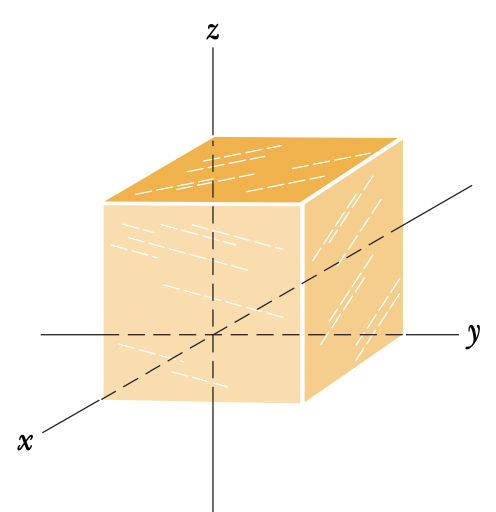
\includegraphics[scale=0.6]{qfig3-1.png}
  \caption{\textbf{문제 2}}
  \label{fig:1}
\end{figure}
\begin{itemize}
\item[(가)] $6.00\,\hat{\bm{i}}$,
\item[(나)] $-2.00\,\hat{\bm{j}}$,
\item[(다)] $-3.00\,\hat{\bm{i}}+4.00\,\hat{\bm{j}}$  
  라면 오른쪽 면을 통과하는 전기장 다발은 각각 얼마인가?
\item[(라)] 정육면체를 통과하는 알짜 전기장 다발(net electric flux)을
  구하여라.   
\end{itemize}


\newpage
{\color{gray} [문제 풀이 쪽]}
\newpage

\noindent {\bf 문제 3 [20pt].} 그림~\ref{fig:2}처럼 질량이 1 mg이고
전하가 $q=2.0\times 10^{-8}$ C로 균일하게 분포되어 있는 작은 부도체
공이 얆고 전하가 균일하게 대전된 부도체 면과 $\theta=30^\circ$의
각을 이루며 부도체 실에 매달려 있다.  
\begin{figure}[htp]
  \centering
  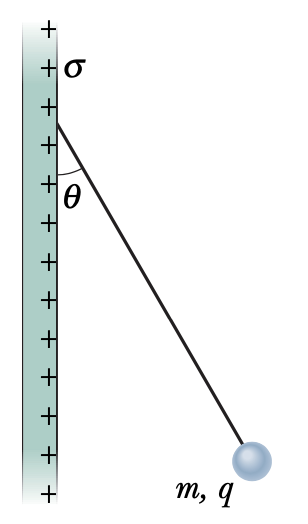
\includegraphics[scale=0.6]{qfig3-2.png}
  \caption{\textbf{문제 3}}
  \label{fig:2}
\end{figure}
이 절연체 판이 무한히 크다고 가정하자. 이와 같은 평형을 만들 수 있는
면전하밀도 $\sigma$를 구하여라. 
\newpage
{\color{gray} [문제 풀이 쪽]}
\newpage

\noindent {\bf 문제 4 [50pt].} 그림~\ref{fig:3}에서 상자 모양의 가우스
면이 $+24.0\varepsilon_0$ C의 알짜전하를 포함하고 전기장
$\vec{E}=[(10.0 + 2.00x)\,\hat{\bm{i}}-3.00\,\hat{\bm{j}}+
  bz\,\hat{\bm{k}}]$ N/C 안에 놓여 있다. 
\begin{figure}[htp]
  \centering
  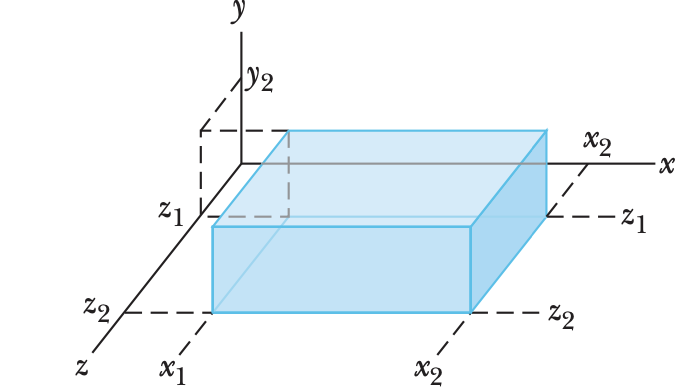
\includegraphics[scale=0.6]{qfig3-3.png}
  \caption{\textbf{문제 4}}
  \label{fig:3}
\end{figure}
$x$, $z$은 미터 단위로
  주어지고, $b$는 상수이다. 밑면은 $xz$평면이고, 윗면은 $y_2=1.00$ m를
  지나는 수평면이다. $x_1=1.00$ m, $x_2=4.00$ m, $z_1= 1.00$ m,
  $z_2=3.00$ m일 때, 상수 $b$는 얼마인가?  
\newpage
{\color{gray} [문제 풀이 쪽]}
\newpage


\end{document}